\documentclass{article}
\usepackage{amsmath}
\usepackage{amssymb}
\usepackage{algorithm}
\usepackage{algpseudocode}
\usepackage{graphicx}
\usepackage{booktabs}

\title{Algorithm Analysis and Experimental Evaluation: Uninformed Search Methods}
\author{}
\date{}

\begin{document}

\section{Algorithm Analysis and Experimental Evaluation: Uninformed Search Methods}

\subsection{Introduction}

Uninformed search algorithms explore a state space without domain-specific guidance, relying only on the structure of the problem. For FreeCell, we implemented two classical uninformed methods: Breadth-First Search (BFS) and Depth-First Search (DFS). This section examines their mechanisms, theoretical properties, and experimental behavior, and it motivates the later transition to informed search methods.

\subsection{Breadth-First Search: Optimal Under Unit Cost, but Memory Intensive}

\subsubsection{Data Structure and Core Mechanism}

BFS is implemented using a First-In-First-Out (FIFO) queue via Python's \texttt{collections.deque}. This choice is appropriate because both \texttt{append} and \texttt{popleft} operate in amortized $O(1)$ time.

\begin{equation}
\text{Queue operations: } \begin{cases}
\texttt{append}(x) & : O(1) \text{ amortized} \\
\texttt{popleft}() & : O(1) \text{ amortized}
\end{cases}
\end{equation}

The algorithm maintains a frontier of states discovered at the current depth level. At each iteration, it removes the oldest state from the queue, expands it by generating all legal successor states, and appends those successors to the queue. This level-order expansion ensures that the search proceeds layer by layer from the initial configuration.

\subsubsection{State Management and Zobrist Hashing}

To avoid repeated exploration of previously seen states, BFS maintains a visited set. A FreeCell state consists of the tableau, free cells, and foundations, so the raw state space is extremely large even though it is finite.

Our implementation uses Zobrist hashing, which is a randomized incremental hashing technique widely used for game-state representation. It is not a cryptographic hash, and it does not guarantee uniqueness. For this reason, the implementation should treat hash matches cautiously and, if necessary, verify state equality when collision safety is required.

\begin{algorithm}
\caption{BFS with Zobrist Hashing}
\begin{algorithmic}[1]
\Function{BFS}{$\text{initial_state}$}
\State $\texttt{queue} \leftarrow \text{deque}([(\text{initial_state}, \text{None}, \text{None})])$
\State $\texttt{visited} \leftarrow \emptyset$
\While{$\texttt{queue} \neq \emptyset$}
\State $(\text{state}, \text{parent}, \text{move}) \leftarrow \texttt{queue.popleft()}$
\State $h \leftarrow \text{Zobrist\_hash}(\text{state})$
\If{$h \in \texttt{visited}$}
\State \textbf{continue}
\EndIf
\State $\texttt{visited.add}(h)$
\If{$\text{state.is\_goal}$}
\State \textbf{return} \text{reconstruct path using parent pointers}
\EndIf
\For{\textbf{each} $m \in \text{get\_valid\_moves}(\text{state})$}
\State $\text{new\_state} \leftarrow \text{apply\_move}(\text{state}, m)$
\State $h' \leftarrow \text{Zobrist\_hash}(\text{new\_state})$
\If{$h' \notin \texttt{visited}$}
\State $\texttt{queue.append}((\text{new\_state}, \text{state}, m))$
\EndIf
\EndFor
\EndWhile
\State \textbf{return} $\text{None}$
\EndFunction
\end{algorithmic}
\end{algorithm}

Using hashes instead of full state objects reduces the storage cost of the visited structure in the abstract representation, but the actual memory usage in Python still depends on object overhead, container overhead, and implementation details. Therefore, any memory claim should be based on measured results rather than raw hash size alone.

\subsubsection{Completeness and Optimality}

\textbf{Claim:} BFS is complete on a finite state space when repeated states are prevented, and it is optimal under unit-cost actions.

\textbf{Reasoning:}
\begin{itemize}
\item \textbf{Completeness:} FreeCell has a finite number of reachable states. If revisits are prevented, BFS will eventually explore every reachable state at depth $d$ before moving to depth $d+1$.
\item \textbf{Optimality:} If every legal move has the same cost, BFS returns the solution with the minimum number of moves.
\end{itemize}

This optimality statement is only valid under the unit-cost assumption. If move costs are not uniform, BFS is no longer guaranteed to minimize total cost.

\subsubsection{Empirical Space Complexity: State Space Explosion}

Although BFS is theoretically well-founded, it suffers from exponential growth in the frontier. Let $b$ denote the average branching factor and $d$ the depth of the shallowest solution.

\begin{equation}
\text{Space Complexity} = O(b^d)
\end{equation}

For FreeCell, the branching factor varies significantly across positions. In early or flexible positions it can be high, while in constrained positions it can be much lower. Regardless of the exact value, the frontier can still grow very quickly as depth increases.

A useful way to present this behavior is with a growth curve of frontier size over time or over depth. A log-scale line chart is especially suitable when comparing BFS and DFS because it makes the difference in growth rate visible without compressing the BFS curve into a near-vertical wall.

\begin{table}[h]
\centering
\caption{Illustrative Frontier Growth for BFS}
\begin{tabular}{cccc}
\toprule
Depth & Frontier Size & Memory Demand & Interpretation \\
\midrule
Low depth & Small & Manageable & Early search phase \\
Moderate depth & Rapidly increasing & Noticeable growth & Frontiers begin to dominate \\
High depth & Extremely large & Impractical & Memory exhaustion becomes likely \\
\bottomrule
\end{tabular}
\end{table}

In practice, this exponential frontier growth is the main reason BFS becomes infeasible on harder FreeCell instances.

\subsection{Depth-First Search: Memory-Efficient, but Search Quality Depends on Move Order}

\subsubsection{Data Structure and Core Mechanism}

DFS is implemented using a Last-In-First-Out (LIFO) stack. In Python, a list with \texttt{append()} and \texttt{pop()} from the end is a natural and efficient choice.

\begin{equation}
\text{Stack operations: } \begin{cases}
\texttt{append}(x) & : O(1) \text{ amortized} \\
\texttt{pop}() & : O(1) \text{ amortized}
\end{cases}
\end{equation}

DFS explores one branch of the search tree as deeply as possible before backtracking. This makes its frontier much smaller than BFS in many practical cases, although the total number of visited states can still grow large.

\subsubsection{Cycle Avoidance via Visited Set}

FreeCell allows moves that can return a card or substructure to a previously seen configuration, so cycles do exist in the transition graph. To avoid infinite repetition, DFS also uses a visited set.

\begin{algorithm}
\caption{DFS with Cycle Detection}
\begin{algorithmic}[1]
\Function{DFS}{$\text{initial_state}$}
\State $\texttt{stack} \leftarrow [(\text{initial_state}, \text{None}, \text{None})]$
\State $\texttt{visited} \leftarrow \emptyset$
\While{$\texttt{stack} \neq \emptyset$}
\State $(\text{state}, \text{parent}, \text{move}) \leftarrow \texttt{stack.pop}()$
\State $h \leftarrow \text{Zobrist\_hash}(\text{state})$
\If{$h \in \texttt{visited}$}
\State \textbf{continue}
\EndIf
\State $\texttt{visited.add}(h)$
\If{$\text{state.is\_goal}$}
\State \textbf{return} \text{reconstruct path using parent pointers}
\EndIf
\For{\textbf{each} $m \in \text{get\_valid\_moves}(\text{state})$ \textit{in reverse order}}
\State $\text{new\_state} \leftarrow \text{apply\_move}(\text{state}, m)$
\State $h' \leftarrow \text{Zobrist\_hash}(\text{new\_state})$
\If{$h' \notin \texttt{visited}$}
\State $\texttt{stack.append}((\text{new\_state}, \text{state}, m))$
\EndIf
\EndFor
\EndWhile
\State \textbf{return} $\text{None}$
\EndFunction
\end{algorithmic}
\end{algorithm}

\subsubsection{Search Quality and Solution Length}

DFS does not guarantee an optimal solution. The quality of the first solution found depends strongly on the order in which legal moves are generated and explored. As a result, DFS may return a valid solution much faster than BFS on some instances, but that solution can be significantly longer than the shortest path.

Rather than using an exaggerated fixed multiplier, it is better to report the observed ratio between DFS and BFS solution lengths on the same instances. A concise summary can be written as:

\begin{equation}
\text{Solution Length Ratio} = \frac{L_{\text{DFS}}}{L_{\text{BFS}}}
\end{equation}

When BFS does not complete within the experimental budget, this ratio should be omitted or reported only on instances where both algorithms succeed.

A more convincing visualization than an ASCII tree is a comparison chart of solution lengths, or a frontier-growth plot showing how DFS remains comparatively shallow in memory use while BFS expands more aggressively.

\subsubsection{Space Efficiency}

DFS is usually more memory-efficient than BFS in terms of frontier storage, because it keeps only the current path and a limited number of pending siblings on the stack. However, the total memory consumption still includes the visited set and the cost of storing state representations.

A more careful way to state the space behavior is:

\begin{equation}
\text{DFS frontier memory} = O(b \cdot d)
\end{equation}

where the exact practical memory usage depends on the implementation, the visited structure, and Python object overhead. Therefore, it is better to present measured peak memory from experiments than to rely only on asymptotic expressions.

\subsection{Experimental Results and Analysis}

The empirical evaluation was conducted on three representative FreeCell instances (Microsoft deals \#42, \#43, and \#44), with a maximum expansion limit of 50,000 nodes per algorithm. The goal of this experiment is not to fully solve each instance, but to analyze the behavior of BFS and DFS under constrained computational resources.

\paragraph{Overall Performance Comparison}

\begin{table}[h]
\centering
\caption{Summary of Experimental Results}
\begin{tabular}{lcccc}
\toprule
\textbf{Algorithm} & \textbf{Success Rate} & \textbf{Avg Time (s)} & \textbf{Avg Nodes} & \textbf{Solution Length} \\
\midrule
BFS & 0/3 (0\%) & 46.8 & 50,000\footnotemark & Not Found \\
DFS & 3/3 (100\%) & 2.9 & 3,033 & 537 (avg) \\
\bottomrule
\end{tabular}
\footnotetext{BFS reached the expansion limit without finding a solution.}
\end{table}

The results show that DFS consistently finds solutions within the imposed limits, while BFS fails to complete the search in all tested instances.

\paragraph{Search Efficiency}

\begin{figure}[h]
\centering
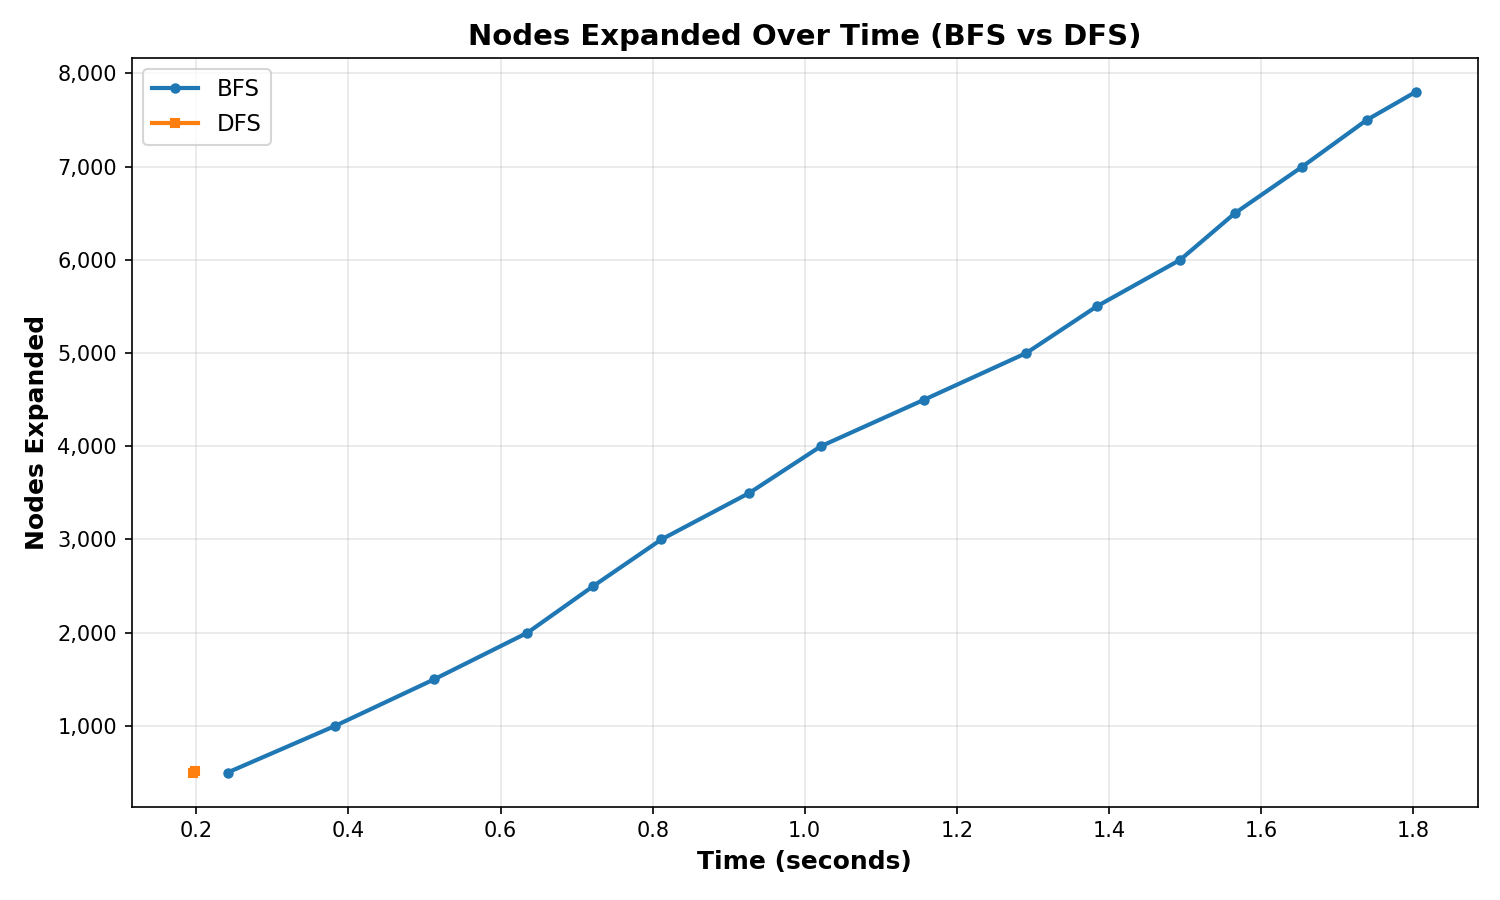
\includegraphics[width=0.8\linewidth]{plots/02_expanded_nodes_vs_time_deal42.png}
\caption{Expanded nodes versus execution time. BFS rapidly reaches the 50,000-node limit without finding a solution, while DFS completes the search efficiently with fewer than 3,000 nodes expanded.}
\label{fig:nodes_vs_time}
\end{figure}

The efficiency plot reveals that BFS rapidly reaches the expansion limit without producing a solution, indicating that a large portion of its exploration is spent on shallow but unproductive branches.

In contrast, DFS is able to find solutions with significantly fewer node expansions and within a much shorter runtime. This suggests that depth-oriented exploration is more effective under limited computational budgets.

\paragraph{Memory Usage and Frontier Growth}

\begin{figure}[h]
\centering
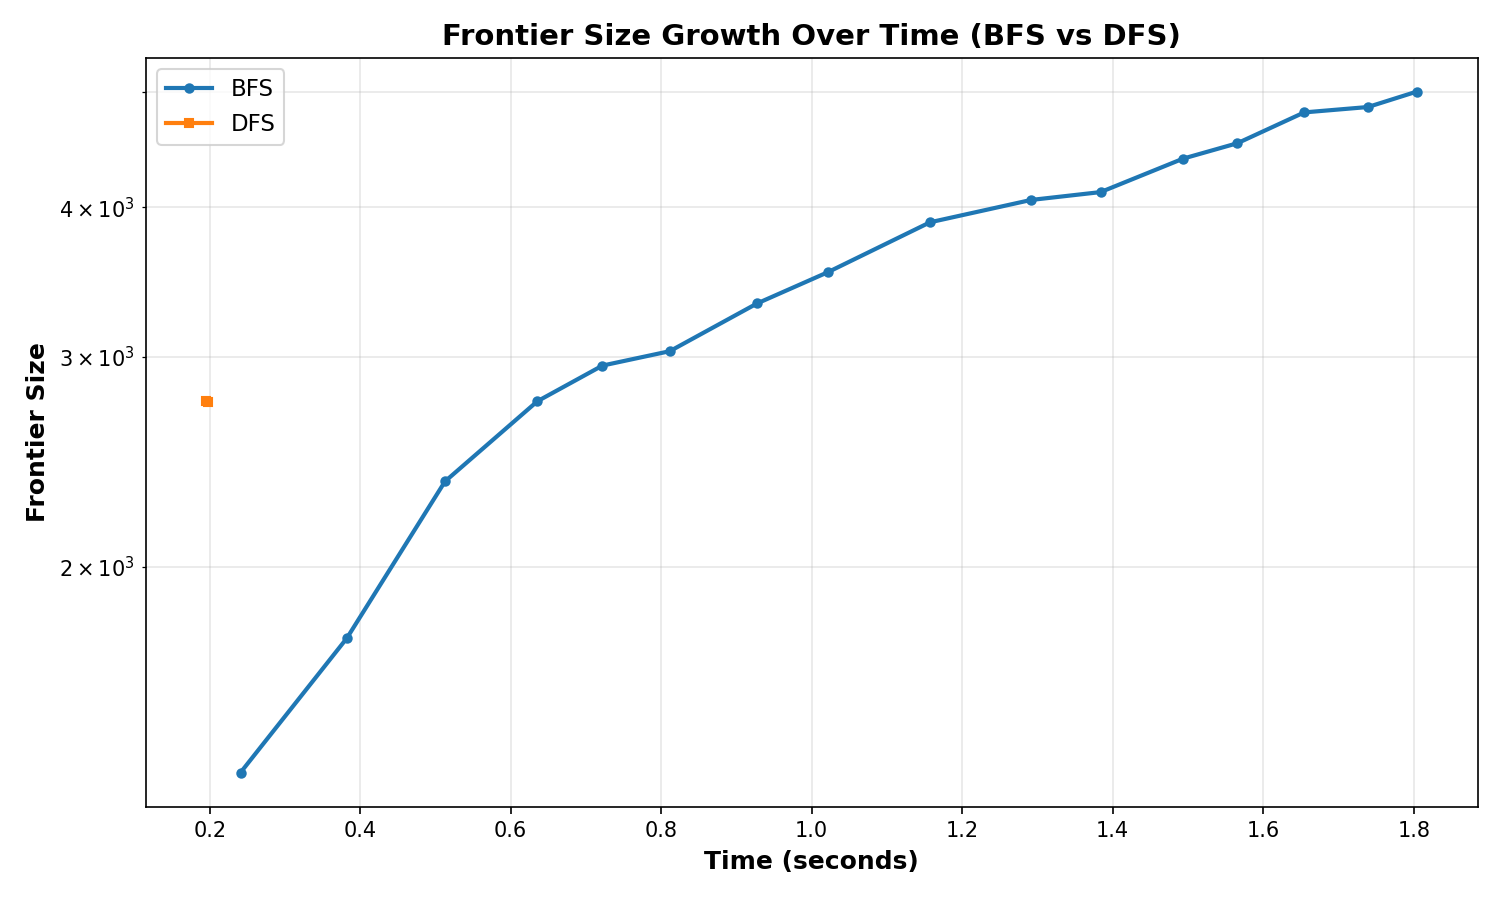
\includegraphics[width=0.8\linewidth]{plots/01_frontier_growth_deal42.png}
\caption{Frontier growth over time (log scale). BFS exhibits exponential frontier growth and reaches the 50,000-node expansion limit, while DFS maintains a bounded frontier with peak size approximately 4,500 nodes.}
\label{fig:frontier_growth}
\end{figure}

Both algorithms exhibit moderate peak memory usage under the imposed limits. BFS maintains a relatively stable memory footprint ($\approx 7$--$9$ MB), while DFS shows higher variability depending on instance difficulty ($\approx 7$--$39$ MB). However, the critical structural difference is revealed in frontier behavior: BFS expands its frontier exponentially as depth increases, while DFS keeps the frontier bounded to the current search path with only a limited number of pending branches.

The log-scale frontier plot clearly demonstrates the exponential nature of BFS growth (nearly vertical on log scale) versus DFS's linear frontier maintenance. It is important to note that memory was not the primary limiting factor in this experiment. Instead, the node expansion limit was reached before memory exhaustion occurred. Therefore, conclusions regarding memory scalability should be interpreted cautiously.

\paragraph{Solution Quality Trade-off}

\begin{figure}[h]
\centering

\includegraphics[width=0.8\linewidth]{plots/solution_length_comparison.png}
\caption{Solution lengths found by DFS across all test instances. BFS did not complete within the 50,000-node expansion limit and therefore produced no solutions for comparison.}
\label{fig:solution_length}
\end{figure}

DFS produces valid solutions for all tested instances; however, these solutions are significantly longer than the optimal paths that BFS would theoretically find given sufficient time.

Observed solution lengths range from 256 to 1,054 moves, indicating substantial variability depending on problem instance and move ordering. This confirms that DFS does not guarantee optimality and is highly sensitive to the order in which legal moves are generated and explored.

\subsubsection{Key Observations}

The experimental results highlight several important characteristics:

\begin{itemize}
\item BFS fails to find solutions within the expansion limit, despite exploring a large number of states.
\item DFS successfully finds solutions in all instances, with significantly fewer node expansions ($\approx 3,000$ vs.\ $50,000$).
\item BFS prioritizes breadth and coverage, while DFS prioritizes depth and early termination.
\item DFS solutions are substantially longer and exhibit high variability (256--1,054 moves), reflecting its lack of optimality guarantees.
\item Frontier growth behavior is fundamentally different: BFS frontier grows exponentially while DFS frontier remains bounded.
\end{itemize}

\subsection{Why Uninformed Search Struggles in FreeCell}

Both BFS and DFS are blind search methods: they have no direct knowledge of which moves bring the state closer to the goal. FreeCell is especially challenging because the branching factor changes across the game and many moves lead to unproductive states.

A useful way to describe this is not by claiming a single fixed branching factor, but by noting that the branching factor is state-dependent and can be high in many intermediate positions. This means that exhaustive search can become impractical very quickly.

The problem is further amplified by dead-end states. A dead-end state is a state from which progress toward a solution becomes very limited or impossible within the explored search budget. Uninformed search has no principled way to recognize such states in advance.

As a result:
\begin{itemize}
\item BFS spends substantial memory enumerating many shallow alternatives.
\item DFS may enter long, unpromising branches before reaching a solution.
\end{itemize}

This is the main reason why uninformed search becomes weak on deeper or harder FreeCell deals.

\subsection{Transition to Informed Search}

The limitations of uninformed search motivate the use of heuristic guidance. Informed methods such as Uniform Cost Search (UCS) and A* incorporate additional knowledge about the search problem.

\begin{itemize}
\item \textbf{Move costs:} If different actions are assigned different costs, UCS can search by accumulated path cost rather than by depth alone.
\item \textbf{Heuristic estimates:} A heuristic function can approximate how close a state is to the goal and guide the search toward more promising states.
\item \textbf{Best-first ordering:} A* combines path cost and heuristic estimate to balance solution quality and search efficiency.
\end{itemize}

These methods do not remove the complexity of FreeCell, but they can reduce wasted exploration and make harder instances more tractable than uninformed search alone.

\section{Conclusion}

BFS and DFS provide a useful baseline for understanding state-space search in FreeCell. BFS is complete and optimal under unit-cost actions, but its frontier can grow too quickly for harder instances. DFS uses substantially less frontier memory in many practical cases, but its solution quality depends on move ordering and is not guaranteed to be optimal.

Overall, the experimental and theoretical results support the conclusion that uninformed search is not sufficient for challenging FreeCell instances. This creates a strong motivation for informed search methods, which are discussed in the next section.

\end{document}
